
\section{Describe the difference between a process and a processor}
A process is a piece of code loaded in random-acccess linked to a stack, heap, an execution context (PID, process state, allocated resources...) and executed by a processor.

A processor is thus the hardware, containing one or more core, each executing one process.


\section{Using 100 processors of 2 Gflops ($2^9$ floating operations per second), what is the performance of the system as measured in Gflops when 10\% of the code is sequential and 90\% is parallelizable?} 
Suppose the runtime on the 100 processors is  $T_P$, what is then the runtime on one processor, $T_1$? We employ Gustafson's law:
\begin{gather*}
T_1 = (f+P(1-f))T_P
\end{gather*}
The speedup factor is now easily determined:
\begin{align*}
S_P &= \frac{T_S}{T_P} \approx \frac{T_1}{T_P} \\
S_P &= f+(1-f)P \\ 
S_P &= 0.1+0.9*100 = 90.1 
\end{align*}

It is roughly 90 times as fast on 100 processors than on one single processor. We conclude that the performance is equivalent to $90.1*2*10^9\approx 180$ .


\section{Is it possible for a system to have a system efficiency ($\eta_P$) of greater than 100\%?}
\[\eta_P = \frac{S_P}{P} = \frac{T_1}{T_PP}  \]

$\eta_P = 100\%$ means that our algorithm performs \textit{P} times faster when using \textit{P} processes instead of one, which can only be achieved if there is no communication between the processes since the communication time is a loss of computation time and if there is no sequential part of the program (i.e. non parallelizable).

Therefore, $\eta_P$ cannot be larger than $100\%$, since it would imply that the sum of the computation time of the \textit{P} processes is lower than the computation time of the sequential algorithm executed by a single process. This would mean that the overall computation time has been reduced, which can only be achievGflopsed if we perform less computations, thus is impossible if we use the same algorithm.
\\
(((Alt. formulation: the time on P processors would be less than one p:th of the time requiered on one processor))) 

\section{Describe a modification of the Parallel Rank Sort method when the number of elements in the list is actually ten times larger than the number of processors in the computer}
When using ten times more elements than the number of processors (and assuming that each processor handle only one process), the most officient solution will be to assign 10 elements to each process.

Assuming that the number of processes P, the rank of the current process p and the array to sort a are already known, the Parallel Rank Sort will then become: \\

\begin{lstlisting}
int i, j, np = n/P
for (i = p*np; i < (p+1)*np; i++) { 
    r[i] = 0;
    for (j = 0; j < n; j++) {
        if (a[j] < a[i]) {
            r[i]++;
        }
    }
}
\end{lstlisting}

\section{You are given some time on a new parallel computer. You run a program which parallelizes perfectly during certain phases, but which must run serially during others.}
\subsection{If the best serial algorithm runs in 64s on one processor, and your parallel algorithm runs in 22s on 8 processors, what fraction of the serial running time is spent in the serial section?}
Now the workload is given, the runtime on multiple processors is therefore:
\[T_P = (f+\frac{1-f}{8})T_S  \] 
We solve for $f$ and obtain:
\[f = \frac{T_P/T_S-1/8}{1-1/8} =  \frac{22/64-1/8}{1-1/8} = \frac{1}{4} \]
Answer: a fourth of the program is serial.

\subsection{Determine the parallel speedup}
The parallel speedup is: \[S_8 = \frac{T_1}{T_8} =\frac{64}{22}\approx 2.9 \]

\subsection{You have another program that has three distinct phases. The first phase runs optimally on 5 processors; this is, performance remains constant on 6 or more processors. The second phase runs optimally on 10 processors, and the third on 15. The phases consume 20\%, 20\%, and 60\% of the serial running time, respectively. What is the speedup on 15 processors?}

\noindent
Let us call the speedup for the phases $S^1,\ S^2 $ and $S^3$. Then the total time on the 15 processors will be:

\[T_P = \frac{0.2T_S}{S^1}+\frac{0.2T_S}{S^2}+\frac{0.6T_S}{S^3}   \]
Whence the speedup, $S_P$
\[\frac{1}{S_P}  =\frac{0.2}{S^1}+\frac{0.2}{S^2}+\frac{0.6}{S^3} \]
Suppose the workload is given and the corresponding serial time is know to be $T_S$. Then the relevant formula is Amdahl's law. Furthermore suppose there is a fraction for each phase that can not be parallelized, then we have the speedup factors as follows:

\begin{gather*}
S^1 = \frac{1}{f^1+\frac{1-f^1}{5}}, \ S^2 = \frac{1}{f^2+\frac{1-f^2}{10}}, \ S^3 = \frac{1}{f^3+\frac{1-f^3}{15}}
\end{gather*}
\[\frac{1}{S_P} = 0.2*(f^1+\frac{1-f^1}{5})+0.2*(f^2+\frac{1-f^2}{10}) +0.6*(f^3+\frac{1-f^3}{15})   \]
As a special case consider $f^1=f^2=f^3 = 0$, then the speedup becoms equal to 10. Just as it should since:
\[\frac{0.2}{5}+\frac{0.2}{10}+\frac{0.6}{15} =\frac{1}{10} \]
If one instead allows the workload to vary one must use Gustafson's law, in which case the speedup becoms:

\[\frac{1}{S_P} = \frac{0.2}{f^1+(1-f^1)5}+\frac{0.2}{f^2+(1-f^2)10}+\frac{0.6}{f^3+(1-f^3)15} \]

Both formulae, of course, yield the same result when $f=0$ or $1$ .\\
Answer: 10
\section{Implementation of the Mandelbrot algorithm using MPI}

\subsection{images}

\begin{figure}[H]
\centering
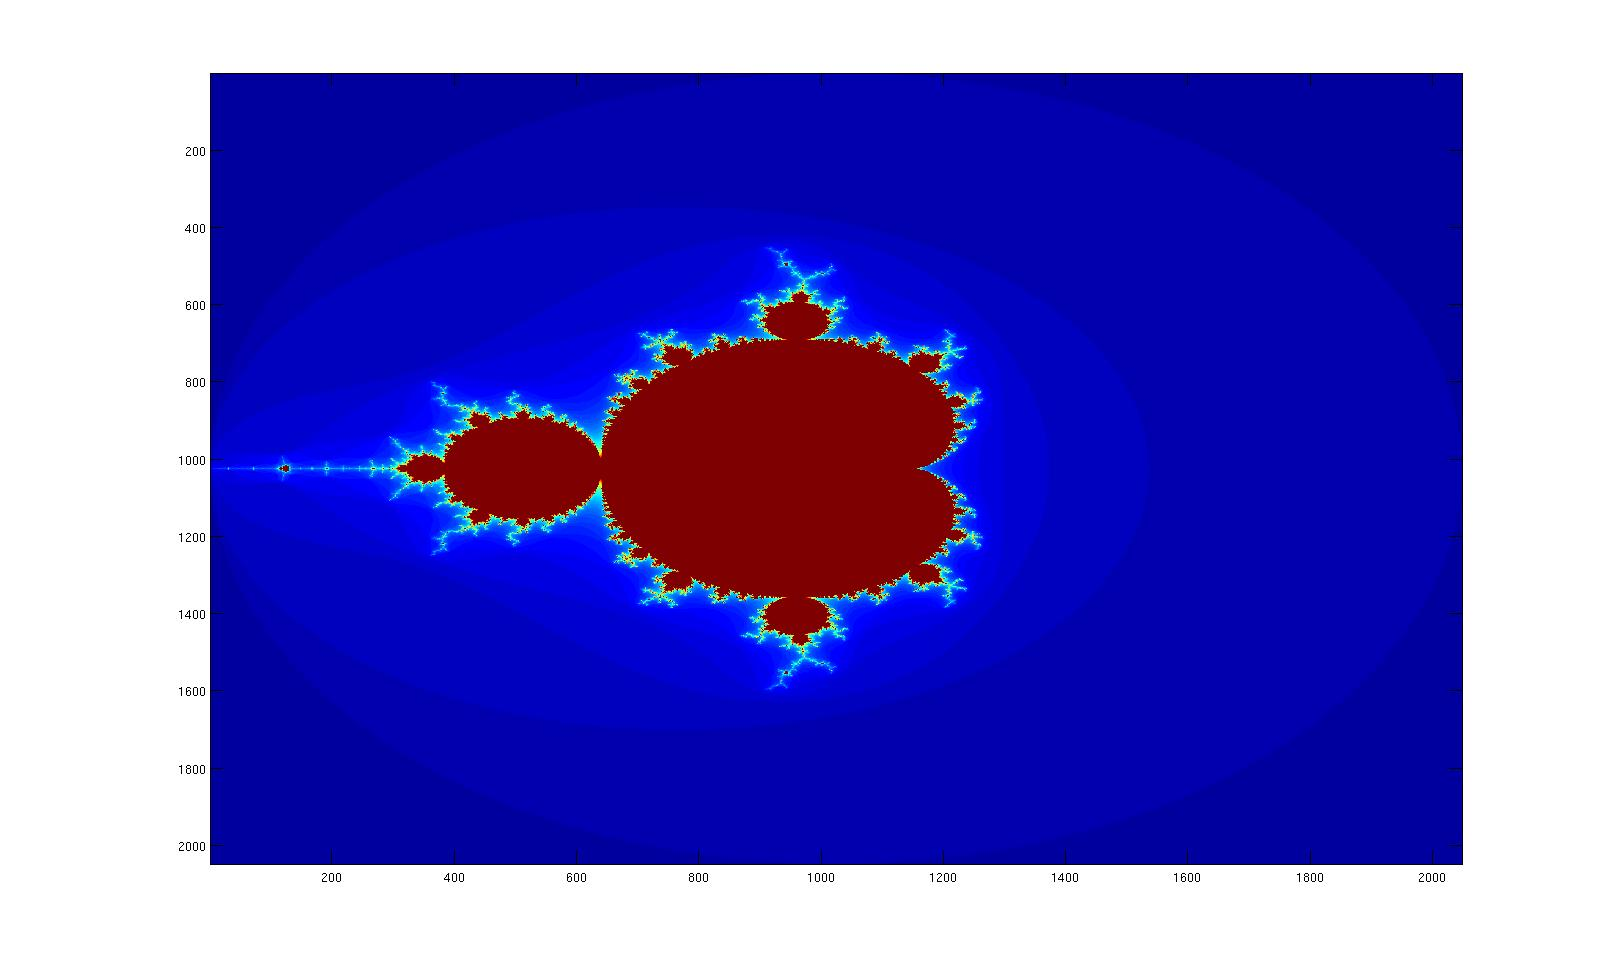
\includegraphics[width=1\textwidth]{img/mandelb.jpg}
\caption{Center is 0}
\end{figure}

\begin{figure}[H]
\centering
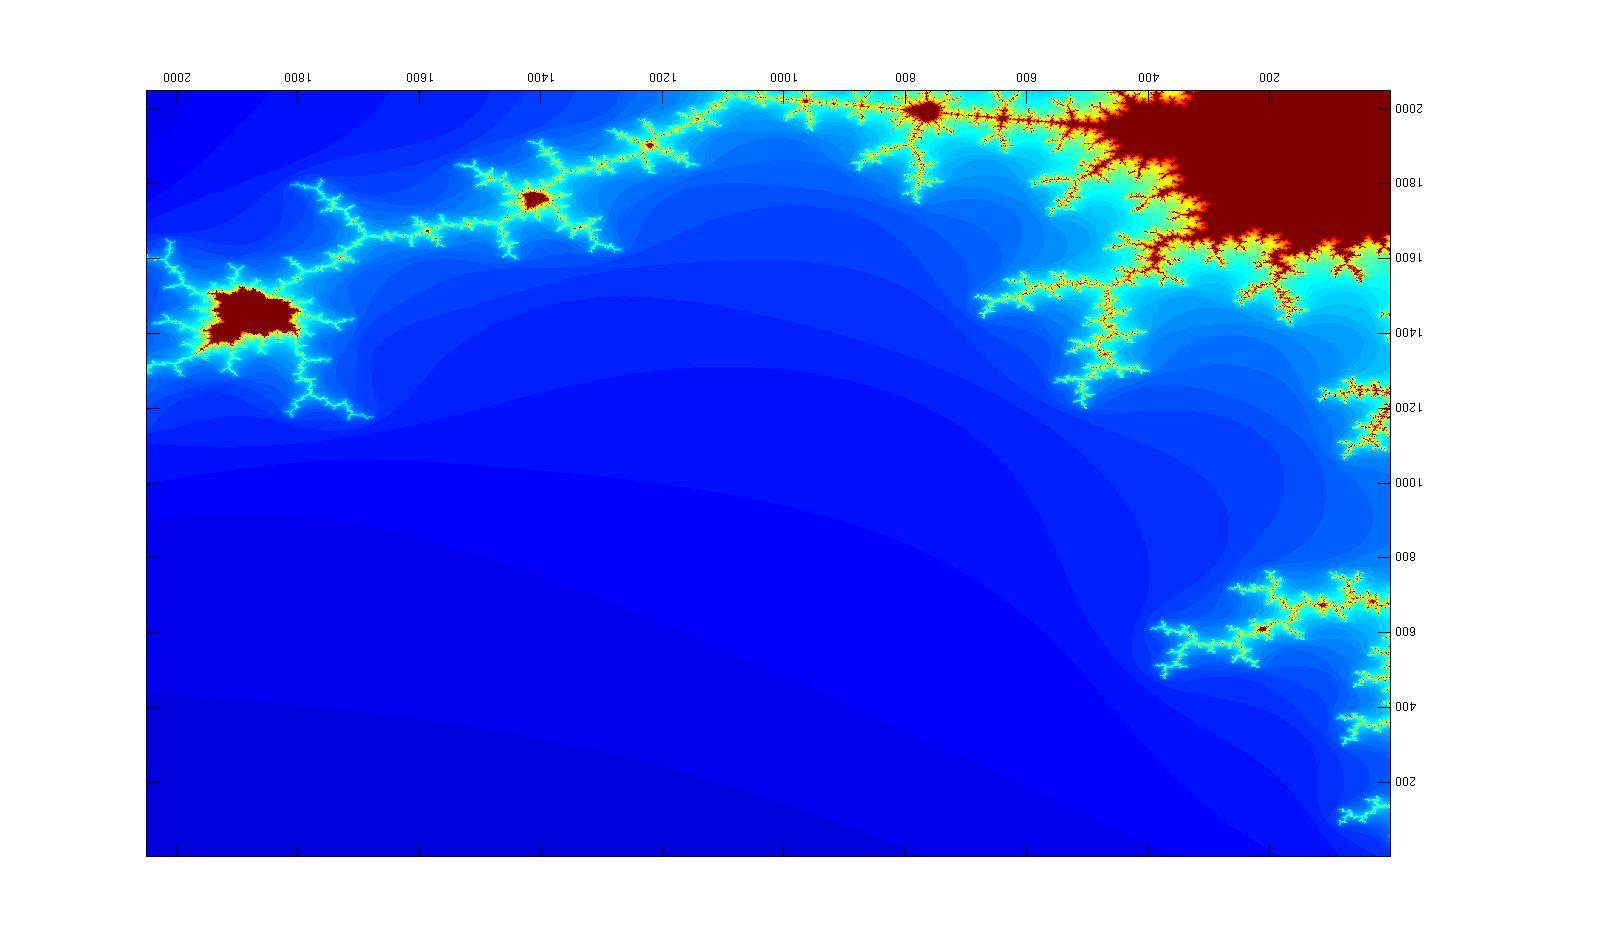
\includegraphics[width=1\textwidth]{img/mandelzoomc01095.jpg}
\caption{Center is -0.2+0.95i}
\end{figure}


\begin{figure}[H]
\centering
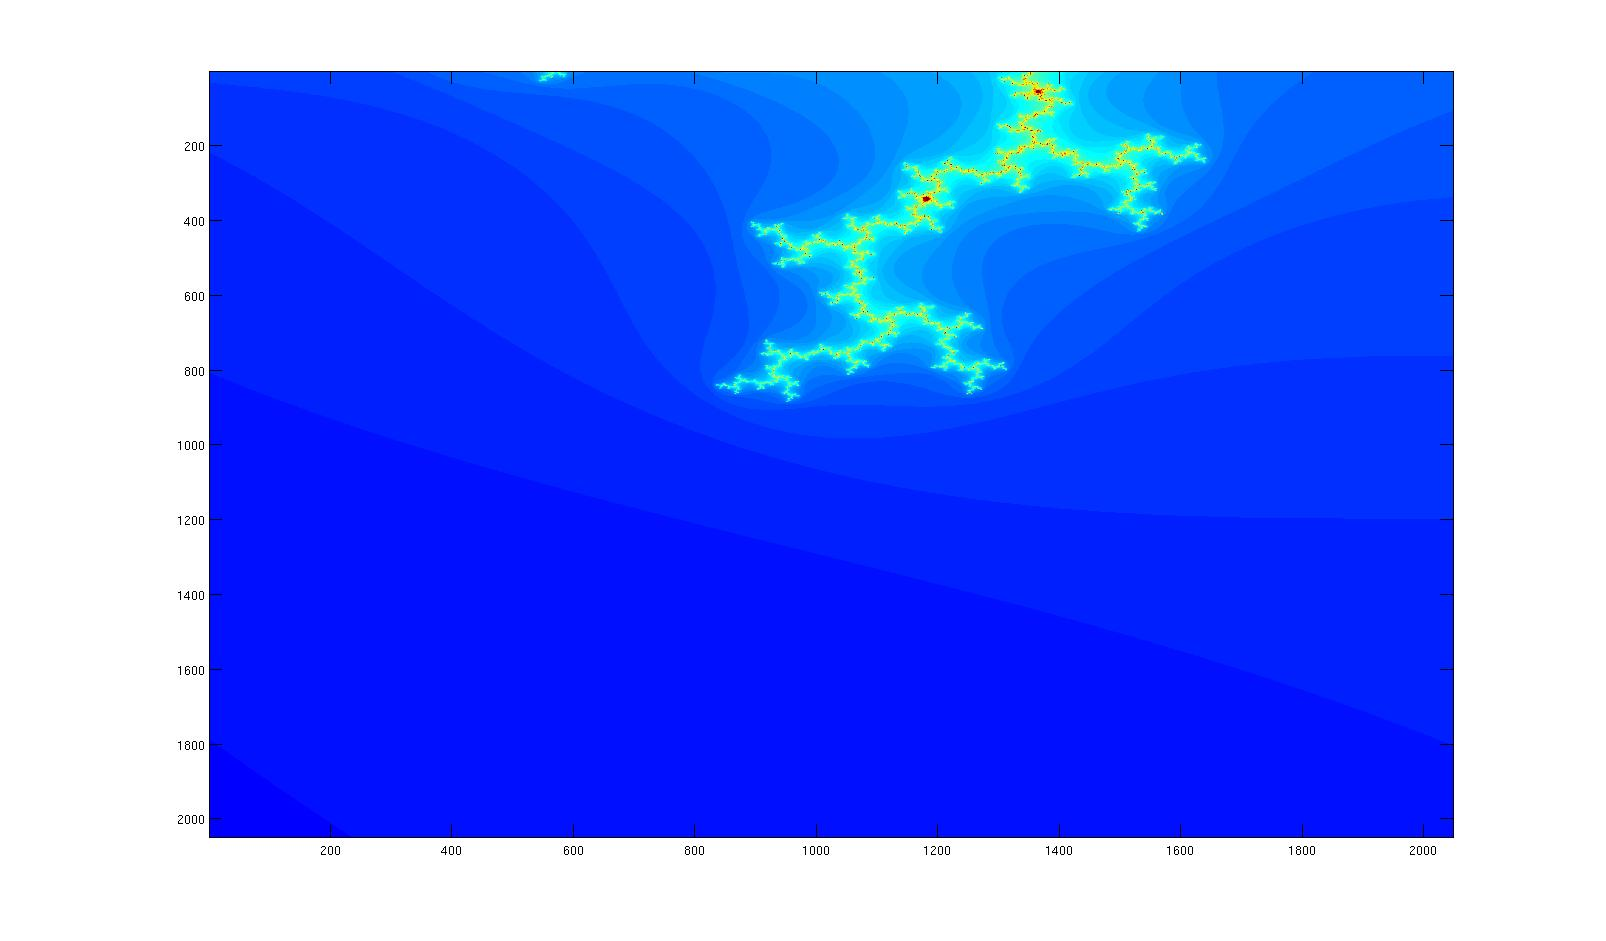
\includegraphics[width=1\textwidth]{img/mandelzoom2.jpg}
\caption{Lower right corner of previous plot magnified 10 times}
\end{figure}
TODO: DEBUG
TODO: INCLUDE FIGURES
